\section{Utilizzo SDK}
\begin{frame}
	\frametitle{Hello Bubble - How to}
%[caption=My Javascript Example]
	\begin{center}
	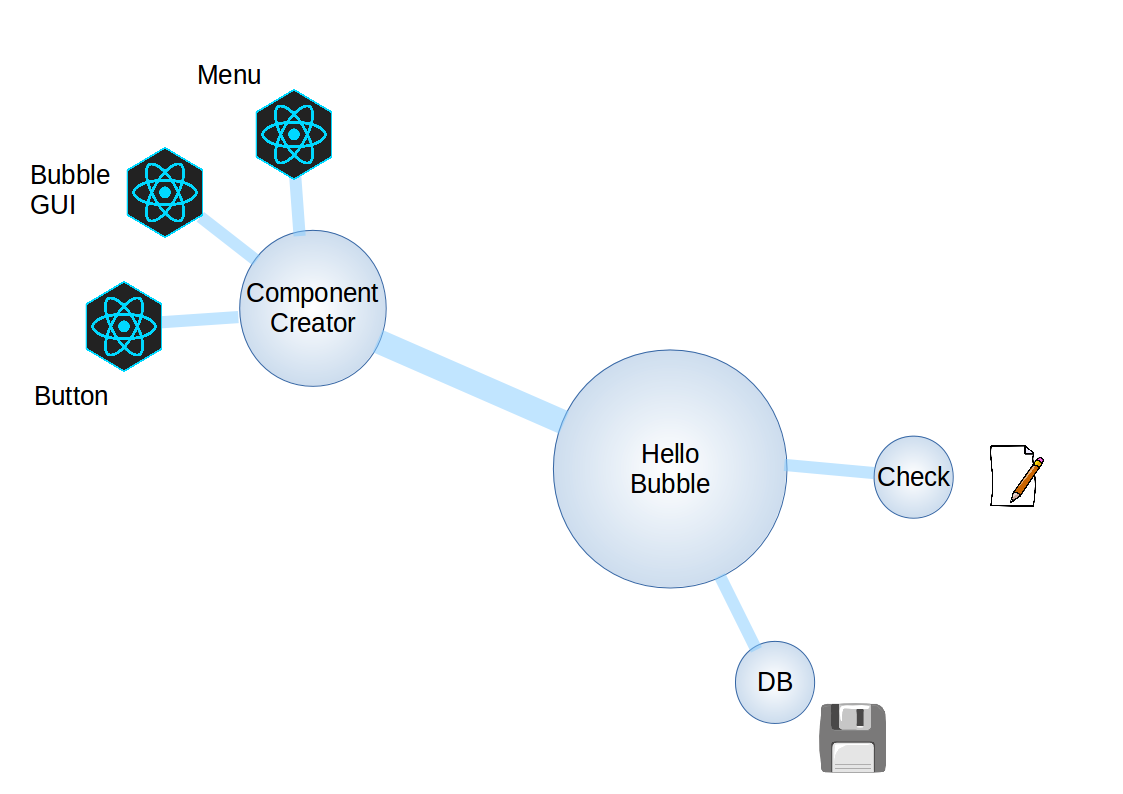
\includegraphics[scale=0.30]{code/bubbleMap.png}
	\end{center}
\end{frame}

\subsection{Hello Bubble - Gui}
\begin{frame}[fragile]
	\frametitle{Bubble Menu}
%[caption=My Javascript Example]
	\begin{center}
	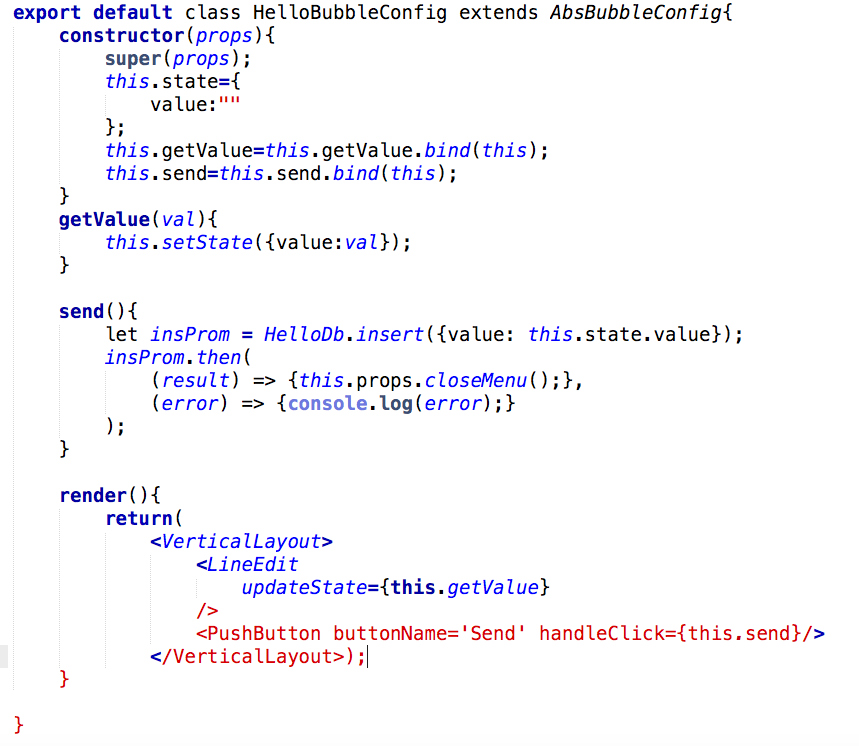
\includegraphics[width=.5\textwidth]{code/hellobubbleconfig.png}
	\vfill
	{
	\vfill
	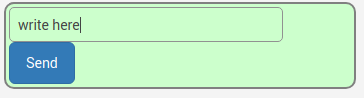
\includegraphics[width=.3\textwidth]{code/config.png}
	\vfill
	}
	\end{center}
\end{frame}

\begin{frame}
	\frametitle{Bubble Button}
%[caption=My Javascript Example]
	\begin{center}
	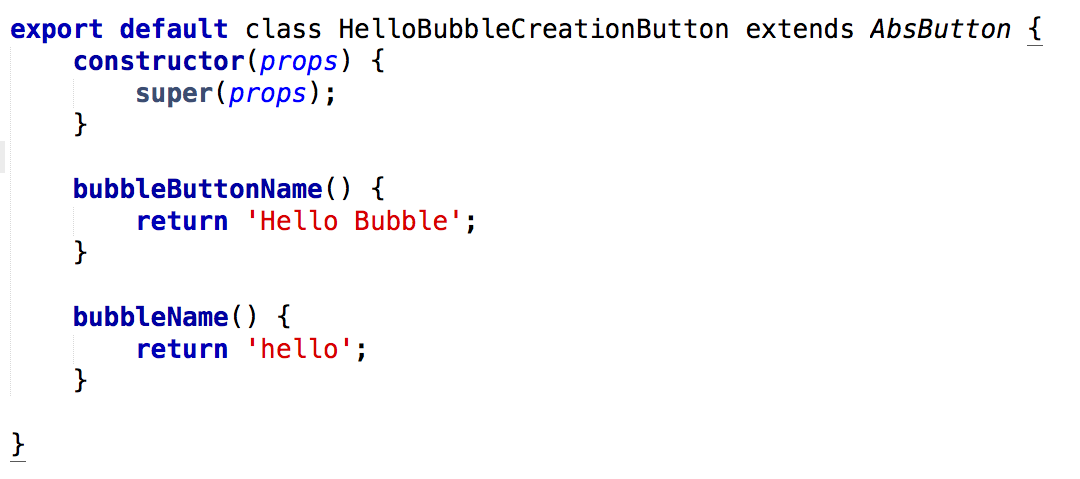
\includegraphics[width=.8\textwidth]{code/hellobubblecreationbutton.png}
	
\includegraphics[width=.3\textwidth]{code/button.png}
	\end{center}
\end{frame}

\begin{frame}
	\frametitle{Bubble Gui}
%[caption=My Javascript Example]
	\begin{center}
	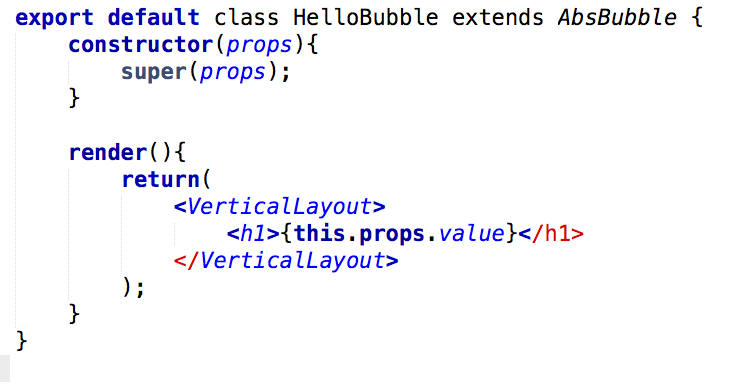
\includegraphics[width=.8\textwidth]{code/hellobubble.png}
	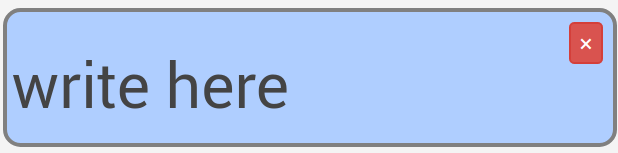
\includegraphics[width=.3\textwidth]{code/bubble.png}
	\end{center}
\end{frame}


\begin{frame}
	\frametitle{Gui managment}
%[caption=My Javascript Example]
	\begin{center}
	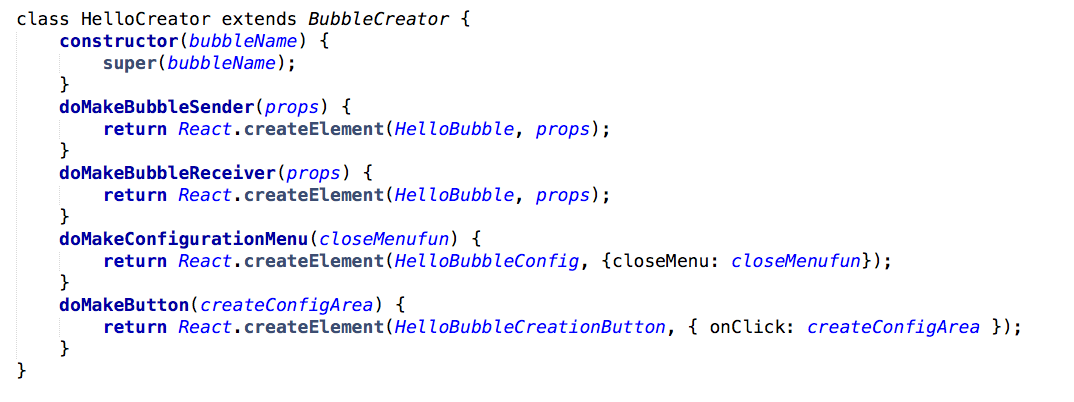
\includegraphics[width=.9\textwidth]{code/hellocreator.png}
	\end{center}
\end{frame}


\subsection{Database and data check}

\begin{frame}
	\frametitle{Database}
%[caption=My Javascript Example]
	\begin{center}
	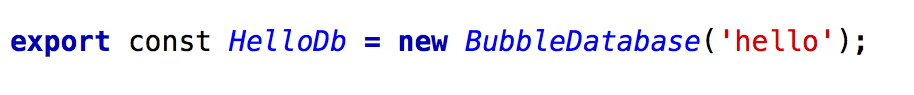
\includegraphics[width=.8\textwidth]{code/helloDb.png}
	\end{center}
\end{frame}

\begin{frame}
	\frametitle{Bubble Check}
%[caption=My Javascript Example]
	\begin{center}
	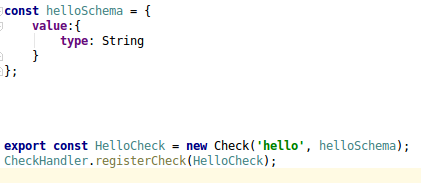
\includegraphics[width=.8\textwidth]{code/hellocheck.png}
	\end{center}
\end{frame}
